對CPU能力的分析表明,只要操作數在寄存器中,處理器就可以同時執行多個操作。可以計算一個相當複雜的表達式,它只依賴於兩個值,所需的時間與將這些值相加所需的時間一樣多。不過,依賴於兩個值的限定是非常嚴重的限制。現在考慮一個代碼示例:

\begin{lstlisting}[style=styleCXX]
for (size_t i = 0; i < N; ++i) {
	a1 += (p1[i] + p2[i])*(p1[i] - p2[i]);
}
\end{lstlisting}

所有代碼都有相同的循環,只是實現更簡單:\texttt{a1 += (p1[i] + p2[i]);}。同樣,\texttt{p1[i]}只是\texttt{v1[i]}的別名,\texttt{p2}和\texttt{v2}也是如此。這個代碼更復雜嗎?處理器可以在一個週期內完成加法、減法和乘法運算,而表達式只依賴於兩個值:\texttt{v1[i]}和\texttt{v2[i]},而這個表達式不能在一個循環中求值。為了明確這一點,我們引入了兩個臨時變量,只是表達式求值過程中的中間結果:

\begin{lstlisting}[style=styleCXX]
for (size_t i = 0; i < N; ++i) {
	s[i] = (p1[i] + p2[i]);
	d[i] = (p1[i] - p2[i]);
	a1[i] += s[i]*d[i];
}
\end{lstlisting}

如前所述,加減的結果\texttt{s[i]}和\texttt{d[i]}可以同時計算。最後一行不能執行,除非已知\texttt{s[i]}和\texttt{d[i]}的值。無論CPU一次可以做多少加法和乘法,但無法計算輸入未知的操作的結果。而這裡,CPU必須等待乘法的輸入準備就緒。第i次迭代需要分兩步執行:首先,必須加減(我們可以同時進行);其次,必須將結果相乘。迭代現在需要兩個週期而不是一個週期,因為計算的第二步依賴於第一步產生的數據:

%\hspace*{\fill} \\ %插入空行
\begin{center}
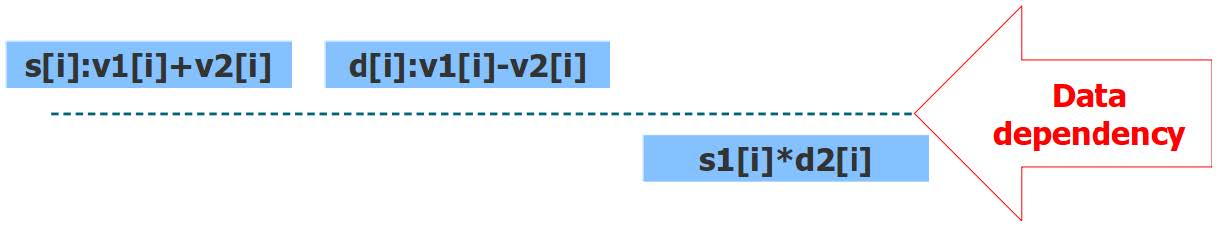
\includegraphics[width=0.8\textwidth]{content/1/chapter3/images/14.jpg}\\
圖3.14 - 循環計算中的數據依賴
\end{center}

儘管CPU有資源可以同時執行這三種操作,但由於計算中的數據依賴,無法使用這種能力。當然,這嚴重限制了我們使用處理器的效率。依賴關係在程序中很常見,硬件設計者想出了有效的解決方案。仔細地看圖3.14,當計算\texttt{s[i]}和\texttt{d[i]}的值時,乘法硬件單元閒置了。不能在更早的時候開始計算乘積,但是可以同時將之前迭代的值\texttt{s[i-1]}和\texttt{d[i-1]}相乘。現在循環的兩個迭代在時間上進行交錯:

%\hspace*{\fill} \\ %插入空行
\begin{center}
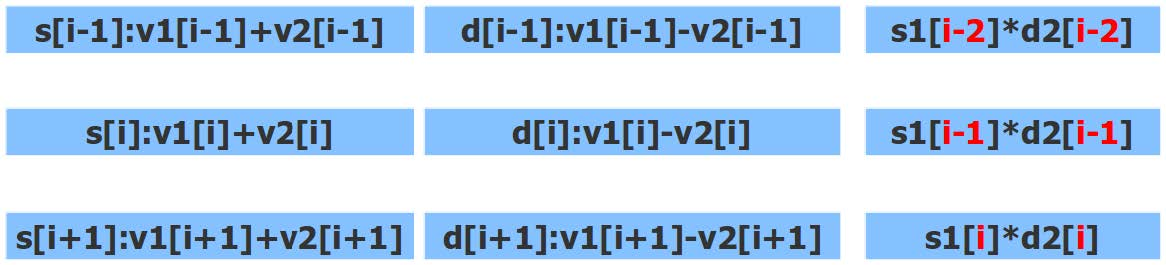
\includegraphics[width=0.8\textwidth]{content/1/chapter3/images/15.jpg}\\
圖3.15 - 流水線:行對應於連續的迭代,同一行中的所有操作將同時執行
\end{center}

這種轉換稱為\textbf{流水線}:將複雜的表達式分解成多個階段,並在流水線中執行。流水線中,前一個表達式的第2階段和下一個表達式的第1階段同時運行(更復雜的表達式將有更多的階段,需要更深層的流水線)。只要有多次迭代,CPU就能像單次乘法那樣快速地計算兩階段加減乘除的表達式:第一次迭代需要兩個週期(先加減,再加減),這無法避免。類似地,最後一次迭代將以乘法結束,同時不能做其他事情,在此期間的所有迭代都會同時執行三個操作。我們已經知道CPU可以同時進行加、減、乘運算,乘法屬於循環內的不同迭代。

可以用一個簡單的基準測試來進行確認。這個測試中,我們將每次循環迭代做一次乘法所花費的時間,與兩步迭代所花費的時間進行比較:

%\hspace*{\fill} \\ %插入空行
\begin{center}
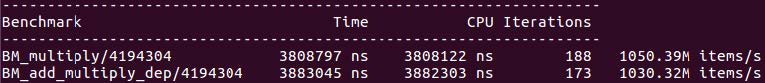
\includegraphics[width=0.9\textwidth]{content/1/chapter3/images/16.jpg}\\
圖 3.16
\end{center}

正如預期,兩個循環在本質上以相同的速度運行。我們可以得出結論,流水線完全消除了由數據依賴引起的性能損失。注意,流水線並沒有消除數據依賴,每個循環迭代仍然必須在兩個階段執行,第二階段取決於第一個階段的結果。通過將不同階段的計算交叉起來,流水線確實消除了這種依賴所致的低效率(至少在理想情況下是這樣的,這也是我們目前所擁有的)。更直接的確認方式,可以從機器碼分析器的結果中看到。同樣,時間軸視圖是最直觀的:

%\hspace*{\fill} \\ %插入空行
\begin{center}
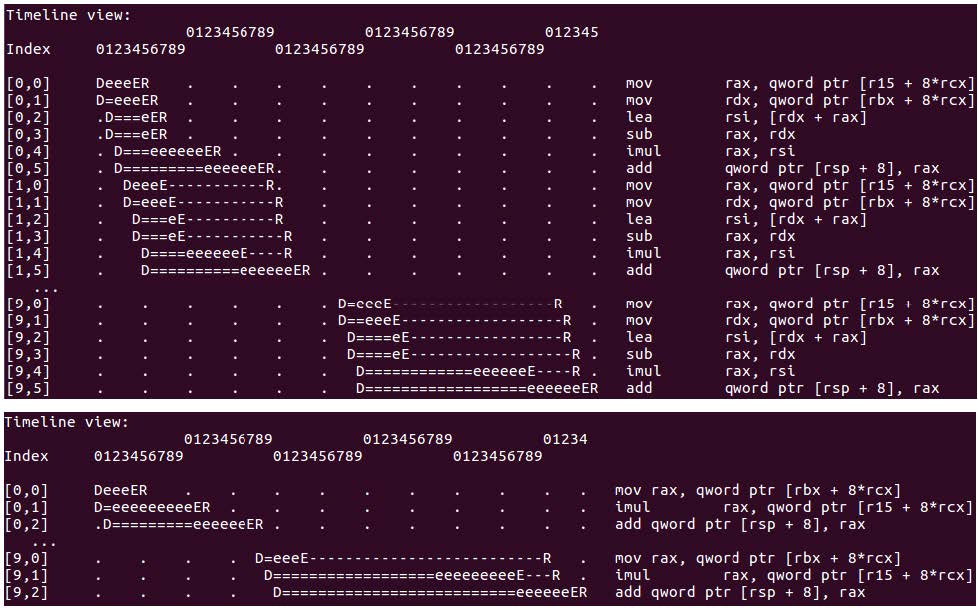
\includegraphics[width=0.9\textwidth]{content/1/chapter3/images/17.jpg}\\
圖3.17 - 流水線的加減乘循環(上)和單乘法循環(下)的時間軸視圖
\end{center}

如您所見,執行任一循環的10次迭代都需要56個週期。時間軸中的關鍵步驟是執行一條指令:\texttt{e}表示執行的開始,\texttt{E}表示執行的結束。流水線的效果在時間軸上清晰可見:循環的第一次迭代開始在第二個循環上執行,指令為[0,0],第一次迭代的最後一條指令是在第18個週期上執行的(橫軸是週期數)。第二次迭代開始在第4個週期執行,兩個迭代之間有明顯的重疊。這就是運行中的流水線,可以看到它是如何提高程序效率的。幾乎每個週期,CPU都在使用它的計算單元執行來自多次迭代的指令。執行一個簡單循環所需的週期與執行更復雜循環所需的週期相同,因此額外的機器操作不需要額外的時間。

本章不打算成為機器碼分析器的手冊,為了更好地理解時間軸和其他信息,讀者們可以自己研究一下它的文檔。不過,有一個問題必須指出來,循環的每次迭代不僅執行相同的C++代碼,也有完全相同的機器碼。因為流水線由硬件完成,而不是編譯器,編譯器只為迭代生成代碼,以及跳轉到下一個迭代所需的操作(或完成後退出循環)。處理器並行執行多條指令,可以在時間軸上看到。經過仔細觀察,有些東西是沒有意義的,例如:圖3.17中的指令[0,4],它在第6和12個週期期間執行,使用CPU的\texttt{rax}和\texttt{rsi}寄存器。在循環第8和9個週期期間執行的指令[1,2]:也使用相同的寄存器,寫進寄存器\texttt{rsi},同時其他指令也會對寄存器\texttt{rsi}進行操作。這是不可能出現的情況,雖然CPU可以使用多個獨立的計算單元同時進行多個操作,但不能同時在同一個寄存器中存儲兩個不同的值。儘管隱藏得很好,但這個矛盾實際上是存在的。在圖3.15中,假設編譯器在所有迭代中只生成一個代碼副本,用來存儲\texttt{s[i]}的寄存器與需要讀取的\texttt{s[i-1]}使用相同寄存器,並且這兩個操作同時發生。

CPU的寄存器比目前看到的要多很多。問題是每次迭代的代碼完全相同,包括寄存器名稱,但是在每次迭代時,必須在寄存器中存儲不同的值。看起來我們的假設和流水線上的實際上情況應該不可能發生,例如:下一個迭代必須等待上一個迭代停止,使用它所需要的寄存器。但真實情況並非這樣,解決這個矛盾的方法使用\textbf{寄存器重命名}的硬件技術。在程序中看到的寄存器名,例如\texttt{rsi},其實不是真正的寄存器名。可以由CPU映射到實際物理寄存器上,所以同名\texttt{rsi}可以映射到具有相同大小和功能的不同寄存器上。

當處理器在流水線中執行代碼時,第一次迭代中指向\texttt{rsi}的指令實際上會使用一個內部寄存器,將其稱為\texttt{rsi1}(這不是它的真實名稱,但寄存器實際硬件的名稱永遠看不到,除非你是處理器設計師)。第二次迭代也有指向\texttt{rsi}的指令,但需要在那裡存儲一個不同的值,因此處理器將使用另一個寄存器\texttt{rsi2}。除非第一次迭代不再需要存儲在\texttt{rsi}中的值,否則第三次迭代將不得不使用另一個寄存器,以此類推。寄存器冊重命名由硬件完成,與編譯器完成的寄存器分配不同(特別是,對分析代碼工具不可見,如:LLVM-MCA或分析器)。最後,循環的多次迭代可以作為一個線性代碼序列執行,就好像\texttt{s[i]}和\texttt{s[i+1]}使用了不同的寄存器一樣。

將循環轉換成線性代碼稱為\textbf{循環展開},這是一種流行的編譯器優化技術。但這次在硬件中完成,對於能夠有效地處理數據依賴關係至關重要。編譯器的角度更接近於源代碼的編寫方式。一次迭代,一組機器指令,通過跳轉到迭代的代碼片段的開頭反覆執行。處理器的角度更像是在時間軸上看到的,一個線性指令序列,每次迭代都有自己的代碼副本,並且可以使用不同的寄存器。

我們還可以觀察到另一個現象,CPU執行代碼的順序實際上與指令寫入的順序並不相同。這稱為亂序執行,它對多線程程序有重大影響。

我們已經瞭解了處理器如何規避數據依賴對執行效率的限制,其解決數據依賴的方法是流水線。然而,故事並沒有在這裡結束。目前為止,設計的用於執行簡單循環的方案缺貌似少了一些東西,因為循環必須在某個點結束。下一節,我們將看到事情會變得多麼複雜,和相應的解決方案。























